\section{Approaches/Designs}

There are many concepts to consider to make effective automated recommendations. Based on prior research in nudge theory, the designs proposed for this research primarily focus on modifying the \textit{locality} and \textit{actionability} of tool recommendations to software developers.

\subsection{Locality}

To better understand how locality impacts the effectiveness of automated recommendations, we examined two separate concepts: \textit{spatial locality} and \textit{temporal locality}. Spatial locality refers to where recommendations are given, while temporal locality focuses on when recommendations are made to potential users.

\subsubsection{Spatial.}

Nudge theory suggests that the placement of options in choice environments, or spatial locality, is an important factor in impacting human behavior and decision-making. For example, the director of food services for a school system with hundreds of thousands of children was able to convince students to eat healthier foods and less junk food by simply changing the arrangement of food choices in the cafeteria, i.e. placing carrots at eye-level instead of French fries. Using this strategy, the director was able to nudge students to adopt better diets and change the consumption of specific food items by up to 25\%~\cite[p.~1]{sunstein2008nudge}. 

We hypothesize location impacts the effectiveness of recommendations to software engineers. For example, developers are more likely to ignore tool suggestions in emails compared to comments in the code. There are many examples of high spatial locality in software engineering. Most integrated development environments have built-in analyzers that highlight syntax errors at the line of code where developers introduce them. Figure \ref{fig:spatial} shows an example of an error reported by the tool  Pylint\footnote{https://www.pylint.org/}, a static analysis tool for Python. Pylint automatically checks for errors and breaches of coding standards by searching for bad patterns and code smells, and uses the red underline to indicate the exact location of an error in the code base. Furthermore, in prior work we developed a code navigation tool \textsc{Flower}~\cite{Flower}. Our results suggest that participants preferred our \textit{in situ} design and we found that it helped improve their efficiency in completing code searching tasks~\cite{Flower}.

\begin{figure*}
\centering
	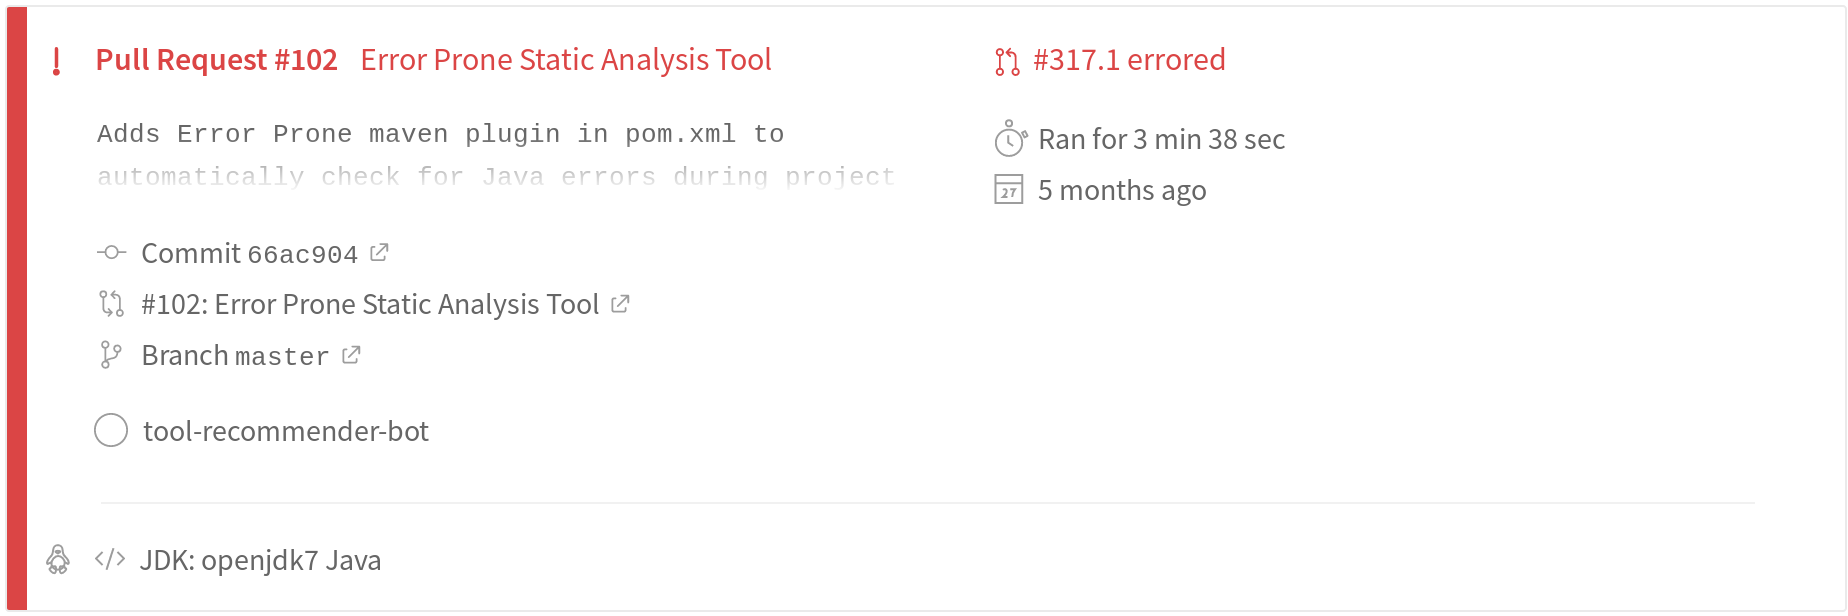
\includegraphics[width=1in]{images/error.png}
	\caption{Example of a high spatial locality}	
	\label{fig:spatial} 
\end{figure*}

\subsubsection{Temporal.}

Research in nudge theory also suggests that timing of recommendations, or temporal locality, plays a role in influencing behavior. One instance of this is the concept of temptation, where Sunstein and Thaler categorize ``hot" and ``cold" states and note that humans are more likely to make certain decisions during hot times~\cite[p.~41]{sunstein2008nudge}. For example, a study found that simply asking people if they intend to purchase a new car within the next six months actually increased purchase rates by 35\%~\cite{morwitz1993intent}. \todo{Better example of timing}

We examine temporal locality to determine if the timing of tool recommendations to software engineers impacts adoption. \todo{SE example}

\subsection{Actionability}

Nudge theory also suggests that actionability, or the ease in which humans can adopt decisions, impacts the choices people make. For instance, a study conducted on Yale seniors found that a lecture on the risks of tetanus, an illness caused by bacteria, was ineffective (3\%) in convincing students to get a shot at the health center. However, providing a campus map to students with the health center circled in the same lecture convinced over nine times more people (28\%) to get the shot~\cite{leventhal1965specificity}. Even though the first group of students knew the location of the health center, adding the map helped students create an actionable plan for getting the shot: allowing them to determine the best route to the health center and how visiting fit in their weekly schedule.

We believe that actionability is another important factor in the outcome of recommendations to software engineers. \todo{SE example}

% \section{Tools}

This section outlines concepts for tools to develop and existing systems to observe for evaluating our approaches in making effective recommendations to software engineers.

\subsection{\TOOL}

% Prior work indicates \textit{active help systems} are more effective for providing suggestions to software users than passive help systems, which require users to deliberately seek help~\cite{FischerActiveHelp}.

% Research shows using software engineering tools can improve the quality of software and the efficiency of developers, but in reality developers rarely use them.

To evaluate approaches for making digital nudges to software engineers for development tool adoption, we developed \TOOL. We aim for researchers to be able to extend \TOOL to recommend useful tools to software engineers. Our system is designed to target developer receptivity in recommendations: the \textit{desire} of programmers to produce high-quality code and their \textit{familiarity} with a project's code base. \TOOL~is an automated recommender system designed to suggest software engineering tools to developers on GitHub\footnote{https://github.com}. We target GitHub users because the code hosting and collaboration website has millions of accounts and public repositories, as well as billions of code contributions from developers\footnote{https://octoverse.github.com/}. \TOOL~recommends development tools by integrating with projects' build configuration. With the rise of continuous integration and deployment, many projects implement build systems to automatically compile, test, and release their software more efficiently~\cite{AkondDeployment}. Integrating projects into the build allows developers to easily integrate new tools into their normal software development workflow. We iteratively modified \TOOL to use different recommendation approaches for nudging developers to adopt different software engineering tools. \TOOL uses a human-presenting GitHub account to recommend tools to developers. Prior work found that bots emulating humans are more effective than bot accounts~\cite{AmongTheMachines}, and we also quickly discovered bot accounts are ineffective for recommendations after our original \TOOL~user\footnote{https://github.com/tool-recommender-bot} was flagged and disabled on GitHub for ``opening multiple unsolicited pull requests in other users' repositories" within a few hours of making recommendations at the beginning of our \tele~study. Our goal is for \TOOL~to integrate numerous recommendation approaches and make software engineering tool recommendations using the most effective nudge type(s) when developers are most receptive to adoption.

\subsection{\SUGGS}

GitHub recently introduced a new feature that allows developers to suggest a change to a project's code modified by a user.\footnote{https://help.github.com/articles/incorporating-feedback-in-your-pull-request/\#applying-a-suggested-change} Suggestions can be utilized during pull request reviews, allowing reviewers to propose changes at the exact line of code in question and developers to easily accept or reject the change. Code reviews are another example of a software engineering action shown to improve code quality, and early feedback on the suggestion feature shows they are very popular and widely adopted by GitHub users. We plan to evaluate the effectiveness of GitHub suggestions as examples of a \location. These situated nudges already have over 100,000 uses on GitHub projects and developers are ``quick to adopt suggested changes" and integrate this feature into their code review process.\footnote{https://blog.github.com/2018-11-01-suggested-changes-update/} This research aims to examine situated nudges in the context of \SUGGS~to determine if the location of recommendations impacts the effectiveness of adoption for developers.

\subsection{nudge-bot}

